\newpage
\subsection{Sensoren}\label{Sensoren}

\begin{wrapfigure}{R}{0.3\textwidth}
\centering
\caption{AS726X}
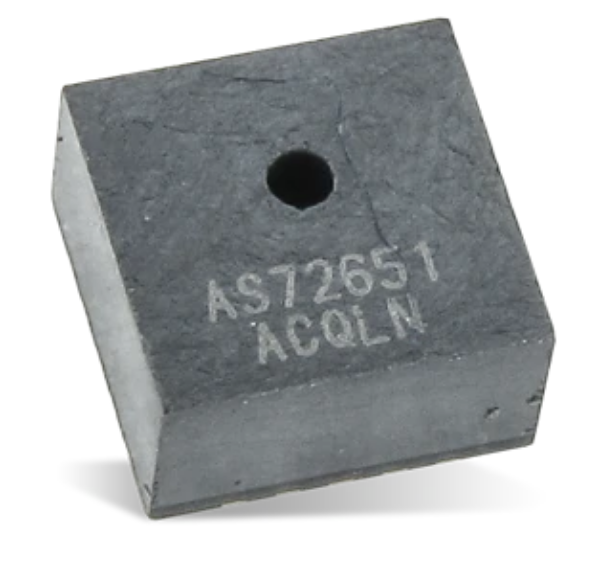
\includegraphics[width=0.25\textwidth]{img/as726X.png}
\label{fig:AS726X}
\end{wrapfigure}

Die Sensoren aus der AS726X Reihe sind in der lage Licht, also elektromagnetische Strahlung zu messen. 
In jedem Sensor sind 6 Photodioden verbaut. 
Vor jeder Photodiode ist ein Silizium-Interferenzfilter montiert, welcher wie ein Bandpassfilter arbeitet, er ist nur für einen bestimmten Ausschnitt des Lichtspektrums durchlässig.
Jeder Baustein enthält einen Analog-digital-Wandler mit 16 Bit Auflösung, der den Strom aus den unterschiedlichen Fotodioden integriert. Nach Abschluss einer Messung wird das integrierte Ergebnis in die entsprechenden Datenregister übertragen.\\
So kann über das beschriebene Sensorarray die farbliche Zusammensetzung des eingestrahlten Lichts erfasst werden.

\begin{figure}[H]
\centering
\caption{Seitenasicht AS726X}
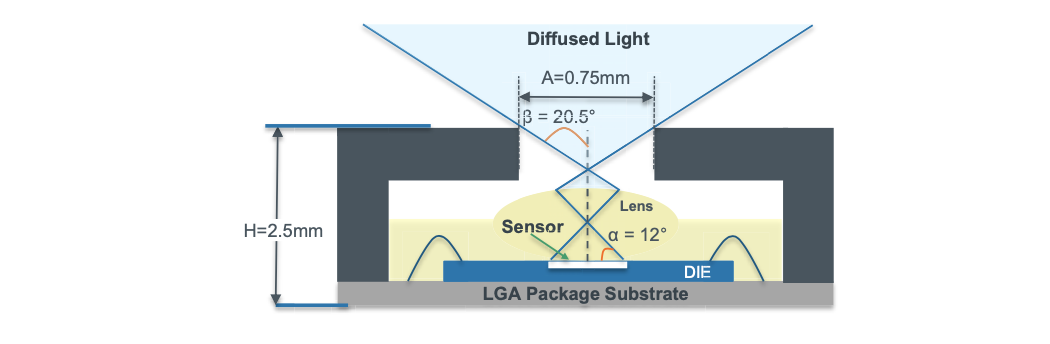
\includegraphics[width=0.9\textwidth]{img/AS726X-seitenansicht.png}
\caption*{Quelle: Datenblatt AS7261}
\label{fig:Seitenasicht-AS726X}
\end{figure}

\noindent Wie in Abb:\ref{fig:Seitenasicht-AS726X} dargestellt, fällt das Licht durch die Öffnung in der Mitte des Sensors ein, eine intern verbaute Linse verteilt das Lich auf die Interferenzfilter. Die Genauigkeit der Filter verändert sich je nach Einstrahlwinkel, daher ist es wichtig, vor den Sensor noch eine Streuscheibe zu montieren.\\
Gemessenen Daten können über UART oder I2C an einen Mikrocontroller übertragen werden, da über UART nur ein Gerät verbunden werden kann, eignet sich aber für diesen Anwendungsfall nur die I2C Schnittstelle.\\
Alle Sensoren erhalten vom Hersteller dieselbe nicht veränderbare I2C Adresse: 0x49. Daher muss ein I2C Translator genutzt werden, welcher es ermöglicht, mehrere Sensoren im gleichen Bussystem zu adressieren(siehe Abschnitt \ref{I2C-Translator}).\\

\noindent Die Modelle unterscheiden sich durch die verbauten Silizium-Interferenzfilter, also die unterscheidbaren Wellenlängenbereiche sowie in der benötigten Peripherie.
Die grundsätzliche Messmethode ist aber immer gleich.
Im Folgenden werden die verwendeten Sensoren AS7261(\ref{AS7261}) sowie der AS7265X(\ref{AS7265X}) beschrieben.

%\begin{wrapfigure}{L}{0.3\textwidth}
%\centering
%    \caption{Seitenasicht AS726X}
% 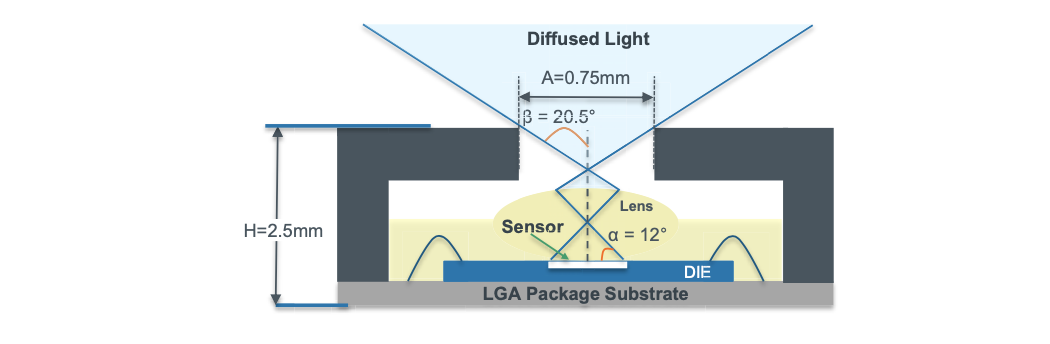
\includegraphics[width=0.7\textwidth]{img/AS726X-seitenansicht.png}
% \caption*{Quelle: Datenblatt AS7261}
%  \label{fig:AS726X}
%\end{wrapfigure}

\subsubsection{AS7261}\label{AS7261}
Das Sensorarray des AS7261 unterscheidet zwischen X,Y,Z,C,D und NIR.
\begin{figure}[H]
  \centering
    \caption{AS7261-Sensor Array}
 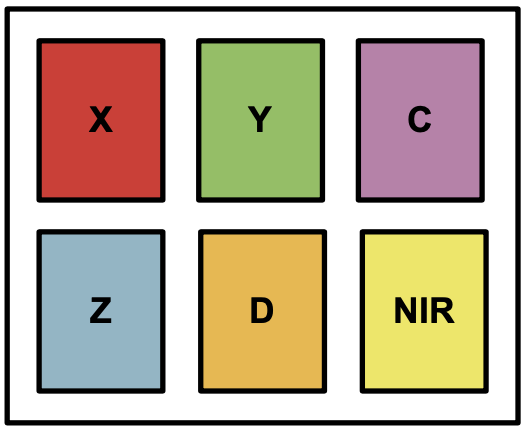
\includegraphics[width=0.4\linewidth]{img/AS7261-Sensor_Array.png}
  \caption*{Quelle: Datenblatt AS7261}
  \label{fig:AS7261-Sensor_Array}
\end{figure}

\noindent Die Ergebnisse des ADC werden direkt, ohne das der Temperaturdrift der Photodioden berücksichtigt wird in die in Tabelle \ref{RAW_Values_AS7261} beschrieben Register geschrieben.


\begin{table}[!ht]
\caption{Your caption.}
\centering
\begin{tabular}{ c c c c}
 kürzel & Bezeichnung & Register & Filtereigenschaften\\
 C & Clear &0x12-0x13& kein Filter \\ 
 D & Dark &0x10-0x11& Lichtdurchlässigkeit des Gehäuses \\  
 NIR & nahes Infrarot &0x0E-0x0F & ????? \\  
 X & X (CIE 1931) & 0x08-0x09 & ????\\
 Y & X (CIE 1931) & 0x0A-0x0B & ????\\  
 Z & X (CIE 1931) & 0x0C-0x0D & ?????\\
\label{RAW_Values_AS7261}
\end{tabular}
\end{table}

Da die Messergebnisse der unterschiedlichen Wellenlängenbereiche den in \ref{TODO} genannten Verzerrungen unterliegen, werden auch noch berichtigte X,Y,Z-Werte bereitgestellt.

\begin{center}
\begin{tabular}{c c c}
 kürzel & Register & Berichtigungs Formel\\
 Cal-X & 0x14:0x17 & ???? \\ 
 Cal-Y & 0x18:0x1B & ???? \\  
 Cal-Z & 00x1C:0x1F & ????? \\  
\end{tabular}
\end{center}

\begin{wrapfigure}{R}{0.6\textwidth}
\centering
\caption{AS7261-Bank Modes}
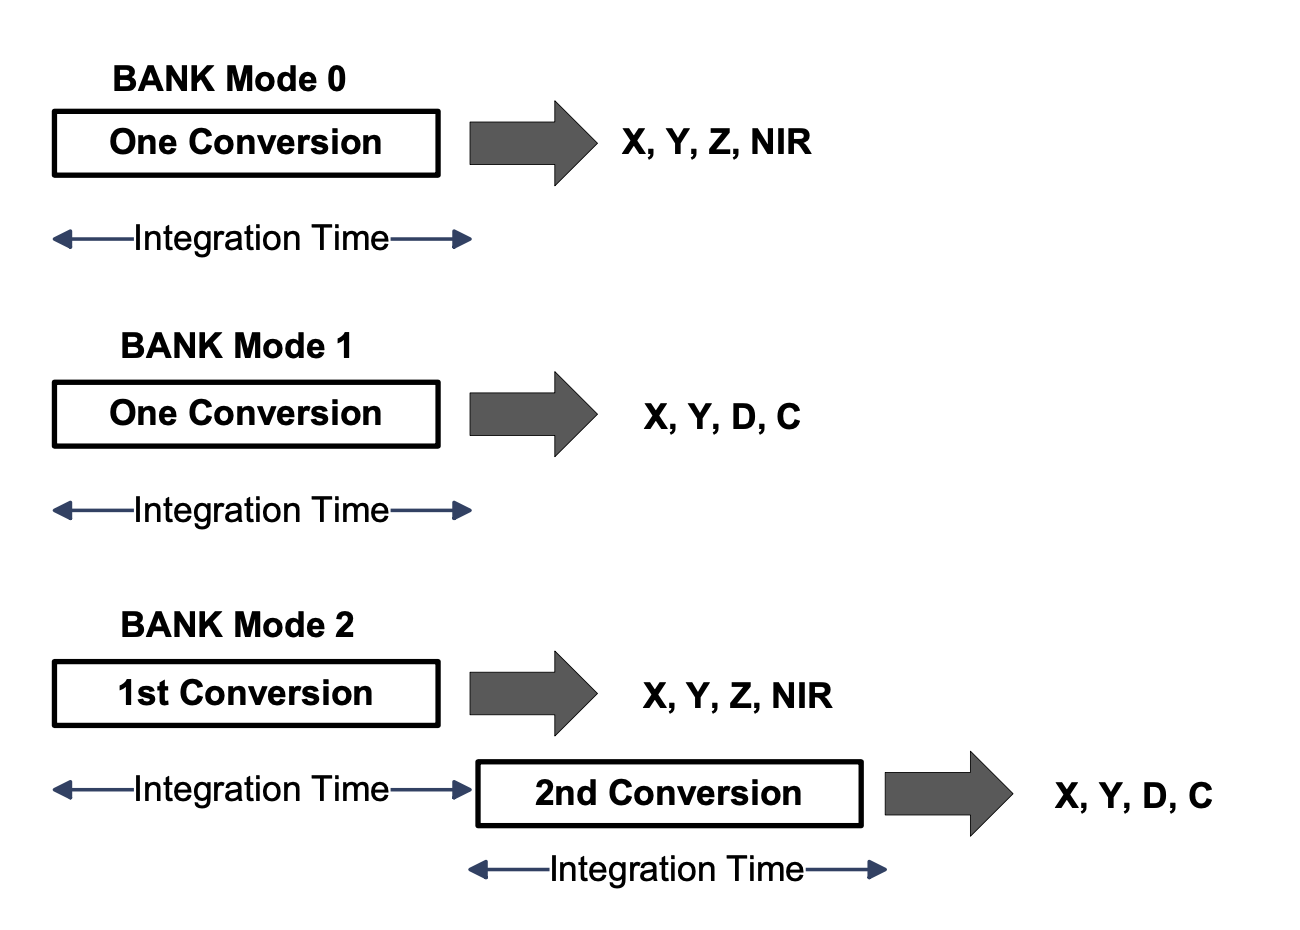
\includegraphics[width=0.5\textwidth]{img/AS7261-Bank_Modes.png}
\label{fig:AS7261-Bank_Modes}
\end{wrapfigure}

\noindent Es gibt 3 sogenannte Bank Modes in denen der Sensor Arbeiten Kann.\\
\textbf{Bank Mode 0}\\
Die Konvertierungen erfolgen kontinuierlich und Daten sind in den I2C-Registern X, Y, Z und NIR verfügbar.\\
\textbf{Bank Mode 1}\\
Die Konvertierungen erfolgen kontinuierlich und Daten sind in den I2C-Registern X, Y, D und C verfügbar.\\
\textbf{Bank Mode 2}\\
Die Konvertierungen erfolgen kontinuierlich, und Daten sind nach zwei Integrationsperioden in den Registern X, Y, Z, NIR, D und C verfügbar. 
In diesem Modus können dauch die kalibrierten, korrigierten Werte auch aus den entsprechenden I2C-Registern abgerufen werden.\\
\textbf{Bank Mode 3}\\
Die Konvertierungen erfolgen nur einmal, und Daten sind wie in Bank Mode 2 nach zwei Integrationsperioden in den Registern X, Y, Z, NIR, D und C verfügbar.
Auch Die kalibrierten, korrigierten Werte auch aus den entsprechenden I2C-Registern können abgerufen werden.
Das DATA RDY-Bit wird auf 1 gesetzt, sobald Daten verfügbar sind.\\
Für diesen Anwendungsfall wird Bankmode 3 verwendet da so an alle angeschlossenen sensoren möglichst gleichzeitig eine messung gestartet werden kann.
Die daten können nach abgeschlossener messung an den NanoPi übertragen werden.


  

\begin{figure}[H]
  \centering
 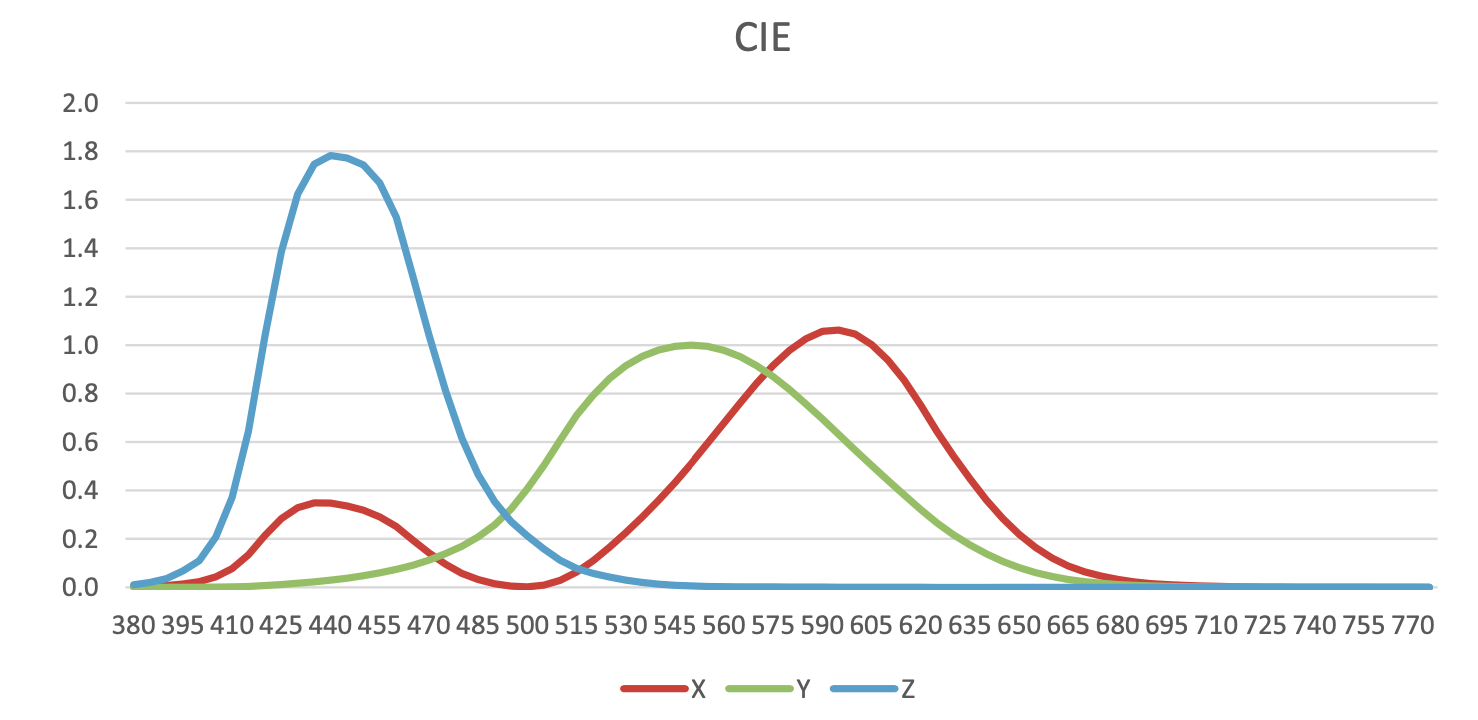
\includegraphics[width=0.6\linewidth]{img/AS7261-Spectral_Responsivity.png}
  \caption{AS7261-Sensor Array}
  \label{fig:AS7261-Sensor_Array}
\end{figure}

\subsubsection{AS7265X}\label{AS7265X}
AS7265X beschreibt AS72651, AS72652 und AS72653 wobei der AS72651 als master für AS72652 und AS72653 fungiert indem er über einen weiteren separaten I2C Bus ihre Daten abfragt und ansonsten wie der AS7261 arbeitet.

\begin{figure}[H]
  \centering
 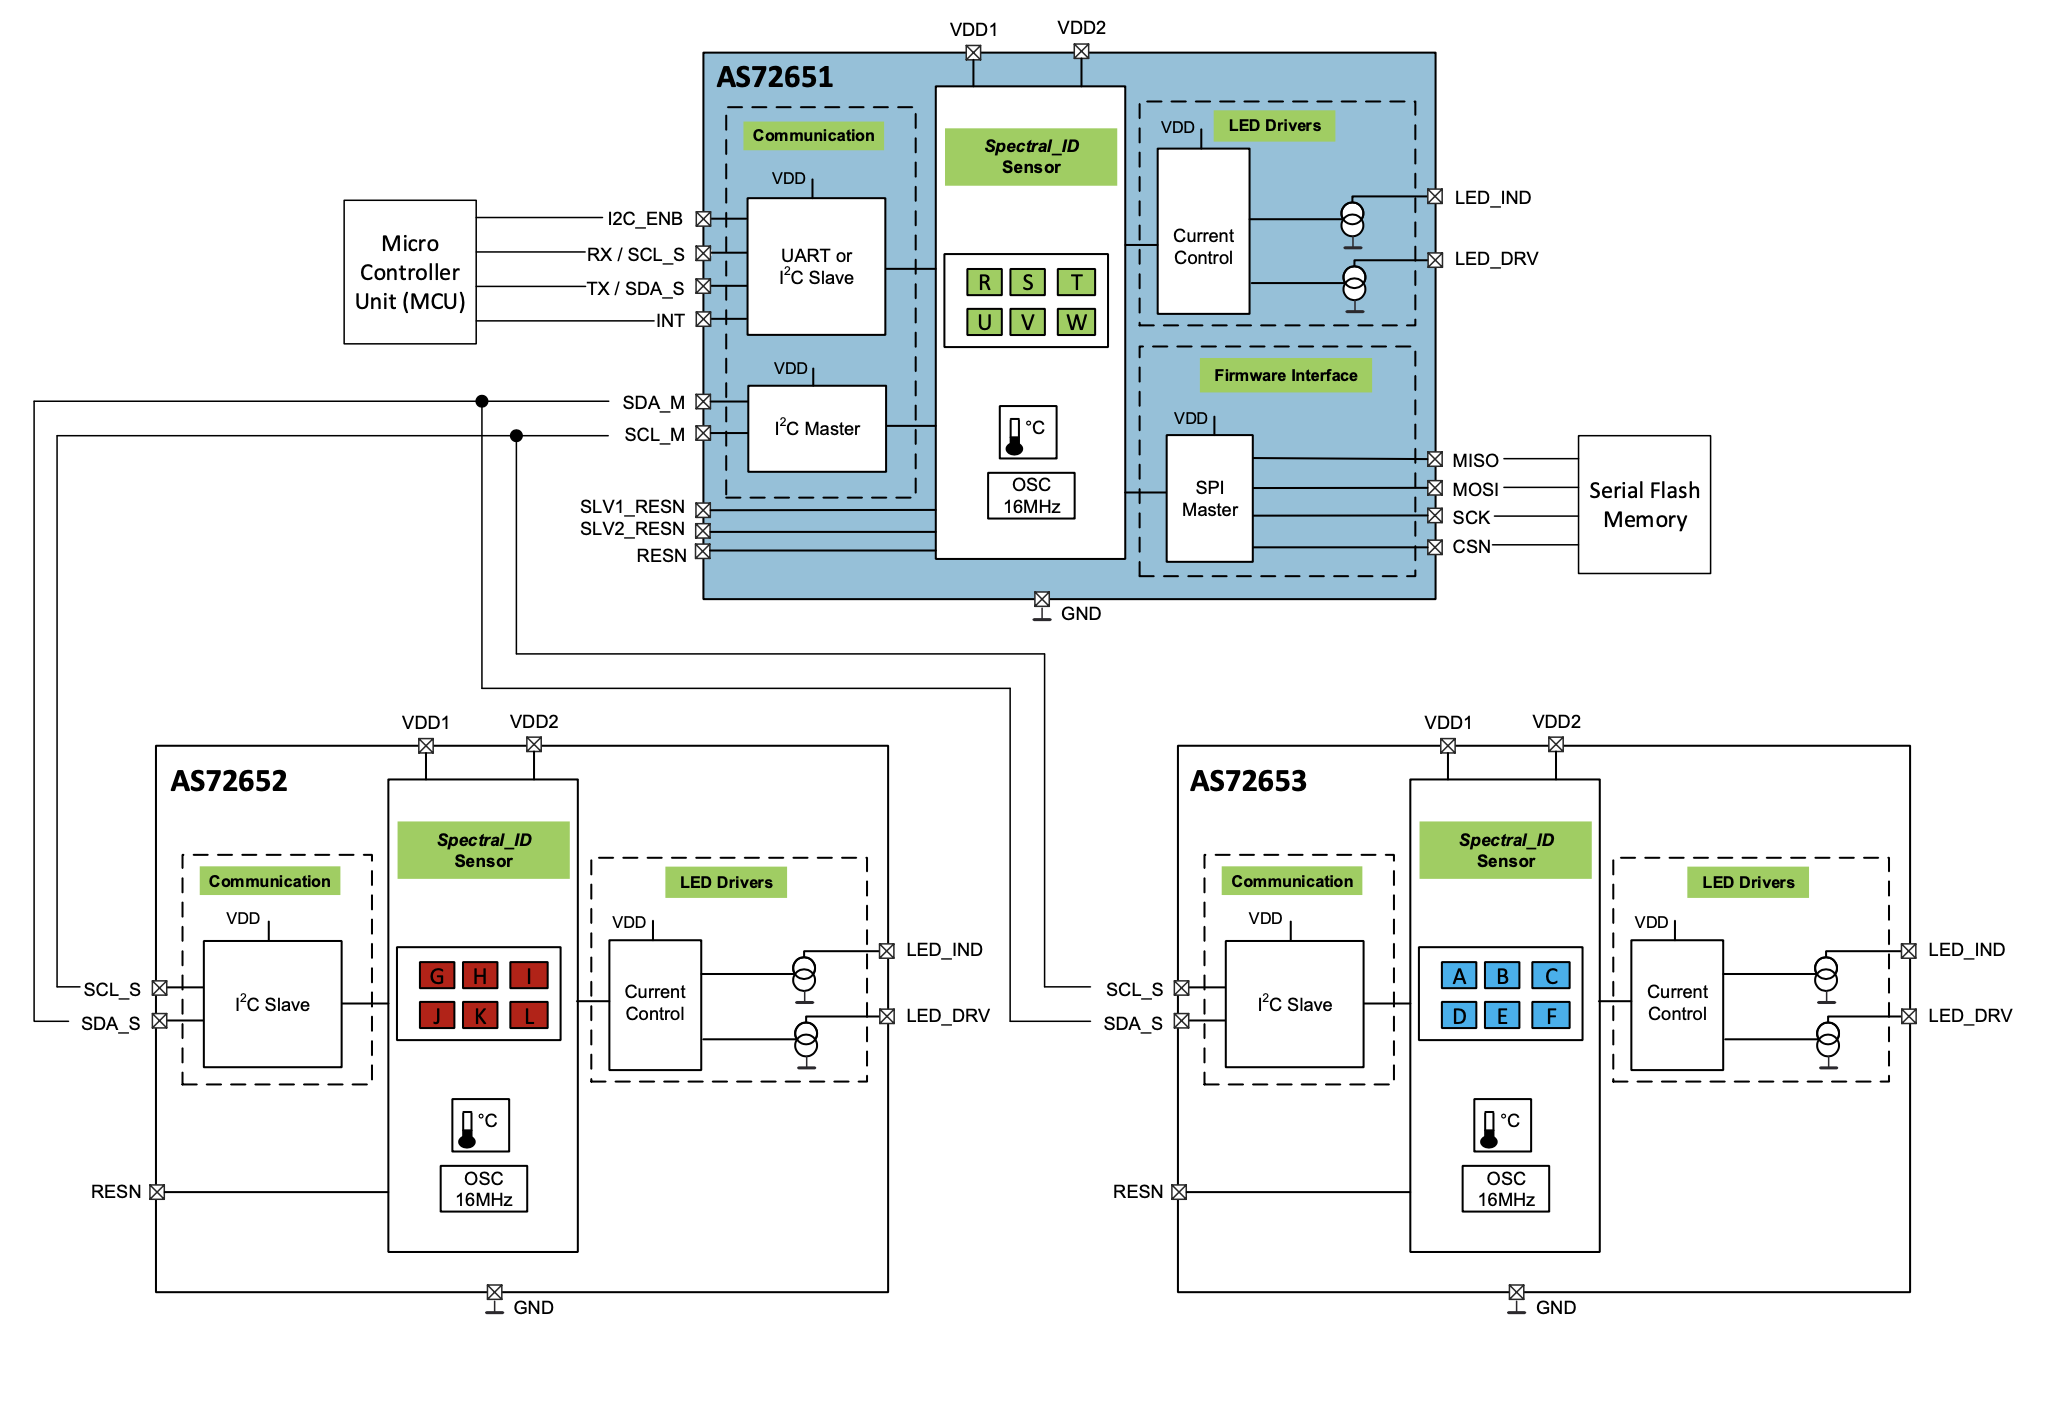
\includegraphics[width=0.9\linewidth]{img/AS7265X-Scematic.png}
  \caption{S7265X-Scematic}
  \label{fig:S7265X-Scematic}
\end{figure}


\begin{figure}[H]
  \centering
 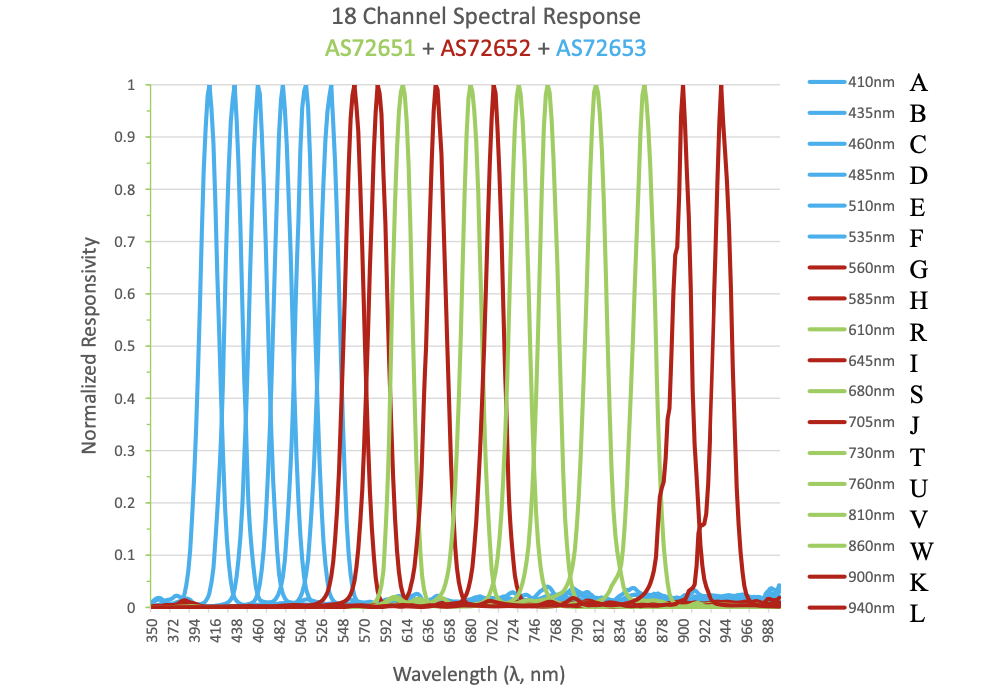
\includegraphics[width=0.9\linewidth]{img/AS7265X-Spectral_Responsivity.png}
  \caption{AS7261-Spectral Responsivity}
  \label{fig:AS7261-Spectral_Responsivity}
\end{figure}
Die drei Sensoren messen in Kombination mit 18 unterschiedliche Photodioden, so können 18 unterschiedliche Frequenz Channel im Bereich zwischen 410 nm und 940 nm mit einer Halbwertsbreite von jeweils 20 nm erfassen.
Die Frequenz Channel sind wie in Abb: TODO zu sehen mit den Buchstaben A-L gekennzeichnet.


\subsection{Mikrocontroller}\label{Mikrocontroller}
Bei der Auswahl des Mikrocontrollers ist die kleine Bauform, ausreichend langlebiger Speicher sowie eine Netzwerkschnittstelle und I2C Anschluss entscheidend.\\
Die abfrage der Messdaten, sowie die Messkonfiguration soll über einen Fernzugriff möglich sein. Die Daten sollen grafisch in einem Webinterface dargestellt werden ohne das eine weitere Server Instanz benötigt wird. Daher eignet sich ein Linux fähiger Einplatinencomputer besser als ein simplerer Mikrocontroller.
Außerdem ermöglicht ein Einplatinencomputer einfache nachträgliche Änderungen ohne das eine komplexe Entwicklungsumgebung eingerichtet werden muss.\\

Der NanoPi NEO2 Black erfüllt alle diese Anforderungen:




\begin{center}
\begin{tabular}{ c c }
 Abmessungen & 4 cm x 4 cm \\ 
 Speicher & eMMC Flash Module Socket \\  
 Anschlüsse & 10/100/1000M Ethernet \\  
 GPIO & UART, I2C, IO \\  
 RAM & 1 GB \\  
 CPU & Allwinner H5 Quad-Core Cortex-A53 \\  
 Preis & TODO     
\end{tabular}
\end{center}
\begin{figure}[H]
  \centering
 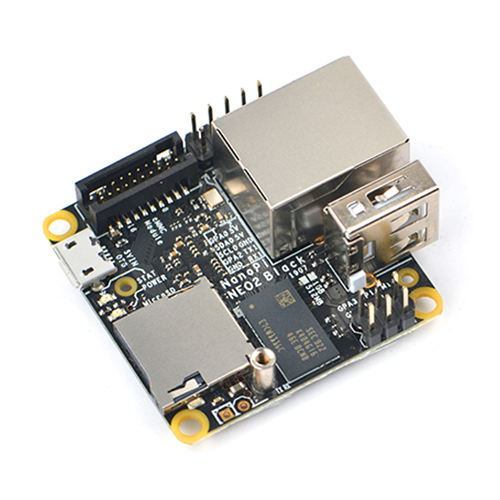
\includegraphics[width=0.5\linewidth]{img/NanoPi_NEO2_Black.jpg}
  \caption{NanoPi NEO2 Black}
  \label{fig:NanoPi_NEO2_Black}
\end{figure}
An den eMMc Socket kann bis zu 128 GB Flash speicher angeschlossen werden.
TODO warum reichen 32 GB.\\
Da eine kabelgebundene Lösung mehr Zuverlässigkeit bietet, wird eine Netzwerkverbindung über Ethernet einer WLAN-Schnittstelle vorgezogen. Es besteht aber die Möglichkeit, einen externen USB WLAN-Adapter nachzurüsten.\\
Die I2C Schnittstelle des NanoPi arbeitet mit 3.3V allerdings wird nur ein 5V und kein 3,3V Output bereitgestellt, daher muss ein steppdown Wandler verwendet werden, um die Sensorboards mit Strom zu versorgen.\\
Die CPU ist für den Anwendungsfall weitaus ausreichend dimensioniert.
In Abbildung \ref{fig:CPU-Performance} ist ein Performancetest zu sehen, die reihen 1-4 beschreiben die prozentuale CPU Auslastung der jeweiligen Prozessorkerne.
Mem beschreibt die Auslastung des Arbeitsspeichers.\\
Für den Performancetest wurde eine Messung an 10 Sensor Boards mit minimalem Messintervall gestartet.
Außerdem wurden gleichzeitig Daten über Grafana exportiert.\\
TODO: Richtiges Bild Performance Test\\
\begin{figure}[H]
  \centering
  \caption{CPU-Performance}
 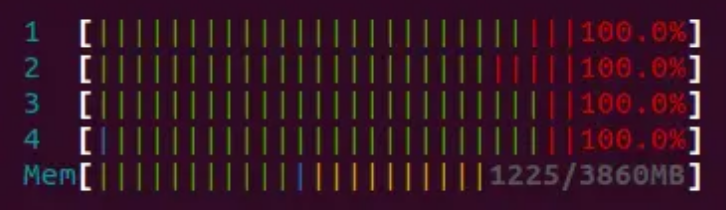
\includegraphics[width=0.7\linewidth]{img/CPU-Performance.png}
  \label{fig:CPU-Performance}
\end{figure}

\subsection{I2C Address Translator LTC4316}\label{I2C-Translator}
Da, wie in Abschnitt \ref{Sensoren} genannt alle Sensoren unter derselben I2C Addresse erreichbar sind, wird ein I2C Translator genutzt, um für eine individuelle Adressierung zu sorgen.\\

\begin{figure}[H]
  \centering
  \caption{I2C-Bus im Messaufbau}
 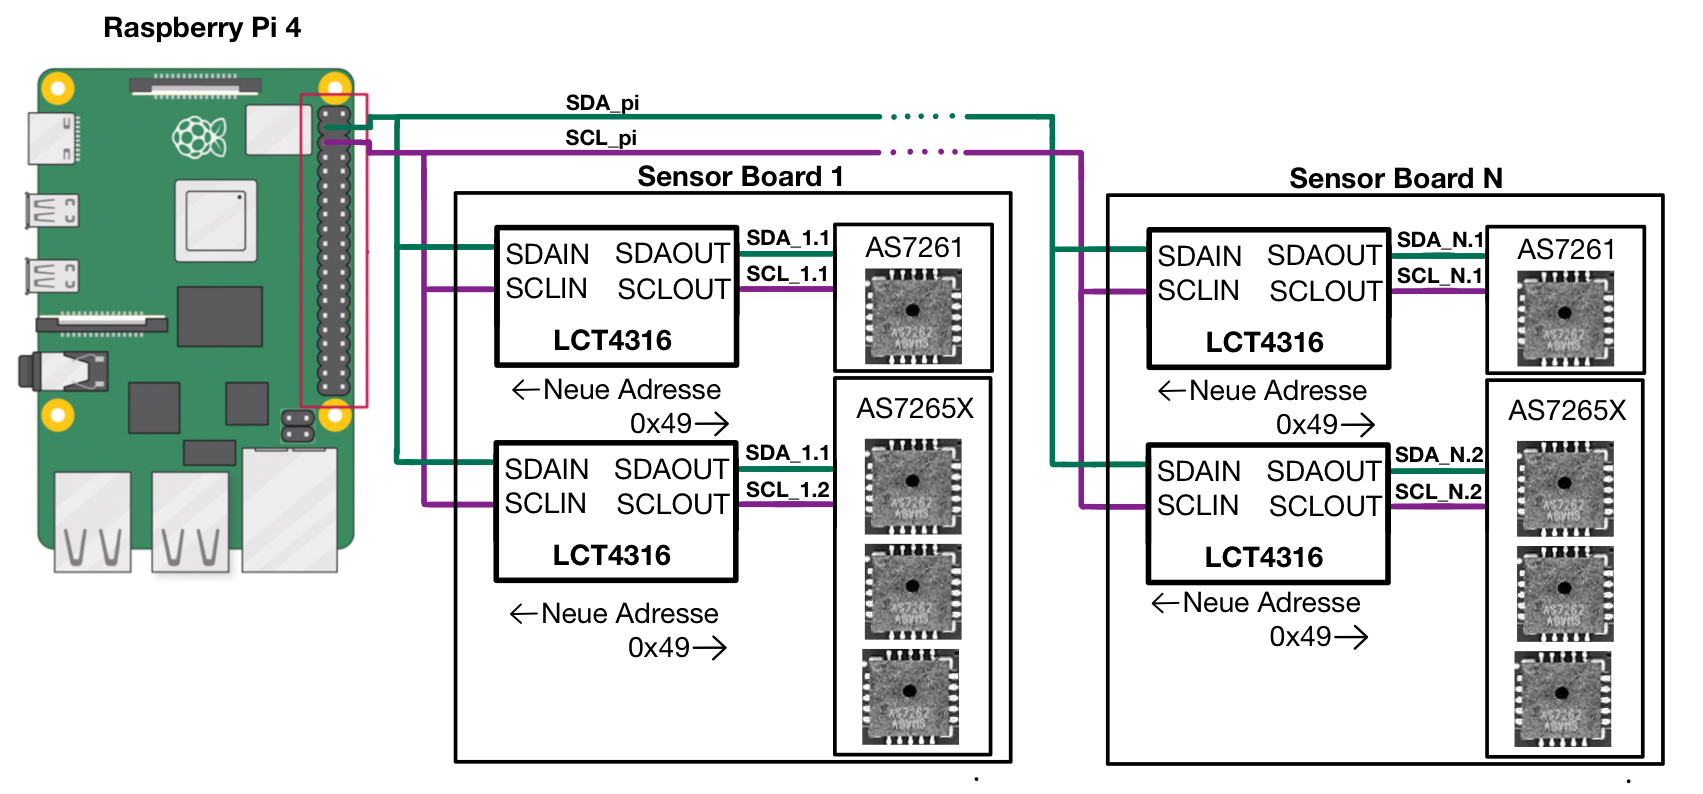
\includegraphics[width=1\linewidth]{img/Adress-Translation}
  \label{fig:adress-translation}
\end{figure}
\noindent Wie in Abb \ref{fig:adress-translation} zu sehen wird für jeden Sensor ein LTC4316 an die Busschnittstelle des Nano-Pi angeschlossen.(SDAIN, SCLIN).\\ 
An jeden LTC4316 wird ein AS7261 oder AS72651 angeschlossen.(SDAOUT, SCLOUT)
Bei Kommunikation vom Nano-Pi zum Sensor wird dann die I2C Adresse mit einem Faktor (Translation Byte) welcher mit diskreten Widerständen eingestellt wird mit Fomel \ref{I2C-translation} verrechnet, um so die Adresse anzupassen.(XORH,XORL).
Um das Translation Byte einzustellen müssen die Widerstände bla,bla und bla wie in Abb \ref{fig:Translation-Byte} am LTC4316 angeschlossen werden.

\begin{equation} 
\label{I2C-translation}
Sensor Adresse\oplus TranslationByte = NeueAdresse
\end{equation}


\begin{wrapfigure}{R}{0.3\textwidth}
\centering
\caption{Translation Byte}

\includegraphics[width=0.25\textwidth]{img/test.jpg}
\label{ffig:Translation-Byte}
\end{wrapfigure}
\bigskip

Beispiel Rechnung\\
$0x49 \oplus 0x01 = 0x48$\\
$0x49 \oplus 0x02 = 0x4b$\\
$0x49 \oplus 0x05 = 0x4c$\\
$0x49 \oplus 0x06 = 0x4f$\\
$0x49 \oplus 0x0A = 0x43$\\
$0x49 \oplus 0x49 = 0x00$\\

\newpage

\noindent In Tabelle \ref{TranslationByte_Lower} und \ref{TranslationByte_Upper} sind die unterschiedlichen Konfigurationen des Translation Bytes aufgelistet.\\
Im Handbuch \ref{Handbuch} ist eine Liste zu finde welche Translation Bytes bereits verwendet werden. Wenn weitere Sensor Boards angefertigt werden ist die Liste dort weiter zu pflegen.

\begin{table}[!ht]
\caption{Untere 4 Bit des Translation Byte}
\label{TranslationByte_Lower}
\centering
\begin{tabular}{c|c|c|c|c|c}
 a3 & a2 & a1 & a0 & $R_{LT}$ & $R_{LB}$\\
 0 & 0 & 0 & 0 & Open & Short \\ 
 0 & 0 & 0 & 1 & 976 & 102\\ 
 0 & 0 & 1 & 0 & 976 & 182\\
 0 & 0 & 1 & 1 & 1000 & 280\\ 
 0 & 1 & 0 & 0 & 1000 & 392\\ 
 0 & 1 & 0 & 1 & 1000 & 523\\ 
 0 & 1 & 1 & 0 & 1000 & 681\\ 
 0 & 1 & 1 & 1 & 1000 & 887\\
 1 & 0 & 0 & 0 & 887 & 1000 \\ 
 1 & 0 & 0 & 1 & 681 & 1000\\ 
 1 & 0 & 1 & 0 & 523 & 1000\\
 1 & 0 & 1 & 1 & 392 & 1000\\ 
 1 & 1 & 0 & 0 & 280 & 1000\\ 
 1 & 1 & 0 & 1 & 182 & 976 \\ 
 1 & 1 & 1 & 0 & 102 & 976\\ 
 1 & 1 & 1 & 1 & Short & Open\\
\end{tabular}
\end{table}

\begin{table}[!ht]
\caption{Obere 3 Bit des Translation Byte}
\label{TranslationByte_Upper}
\centering
\begin{tabular}{c|c|c|c|c|c}
 a6 & a5 & a4 & $R_{LT}$ & $R_{LB}$\\
 0 & 0 & 0 & Open & Short \\ 
 0 & 0 & 1 & 976 & 102\\ 
 0 & 1 & 0 & 976 & 182\\
 0 & 1 & 1 & 1000 & 280\\ 
 1 & 0 & 0 & 1000 & 392\\ 
 1 & 0 & 1 & 1000 & 523\\ 
 1 & 1 & 0 & 1000 & 681\\ 
 1 & 1 & 1 & 1000 & 887\\

\end{tabular}
\end{table}

\subsection{Companion Flash}
Die Sensoren AS7261 und AS72651 benötigen einen flash speicher von welchem sie ihre Firmware laden können.
Die jeweilige Firmware von AMS wird mithilfe von Flashcat-USB, einem USB Memory Programmer über das SPI Protokoll auf den den Flash Speicher übertragen.
Der AT25SF041-SSHD-B wurde aus der von AMS bereitgestellten liste kompatiebler Flash speichern ausgewählt da er am günstigsten ist. 



